\documentclass{article}


\usepackage[charter]{mathdesign}
\usepackage{fullpage}
%\usepackage{amssymb}
\usepackage{amsmath}
\usepackage{verbatim}
\usepackage{ifthen}
\usepackage{url}
\usepackage{xspace}
\usepackage{graphicx}
\usepackage{subcaption}
\usepackage{amsthm}
\usepackage{calrsfs}
\usepackage[hidelinks]{hyperref}
\usepackage{authblk}
\usepackage[show]{notes}
\usepackage{minted}


\title{ELEC-E8125 \\
        Reinforcement Learning Project} 
\author{  Ananth Mahadevan\\
\and
Alexandru Dumitrescu\\
}
% \affil{Department of Computer Science, Aalto University\\

\date{}
\begin{document}
\maketitle
\clearpage
\tableofcontents
\clearpage

\section{Introduction}
\label{sec:introduction}
Something


\section{Literature Review}
\label{sec:external}
Although the game of Pong is much simpler than traditional board games such as chess, the number of states in a game are still exponentially large. This is due to the position of both the players' paddle and the location of the ball (even though the models are trained on pixels, the number of unique image-states can be directly determined by the number of unique position combinations of the 2 paddles and the ball). Hence, we conclude functional approximation methods are prefered to tabular methods in this case.

\medskip
\noindent
We then turn our attention to functional approximation representation methods, which seek to use statistical models (in this case neural networks) to approximate the Q-value table in Deep Q-networks or the policy and critic values in the actor critic method. This also increases the sample frequency of the methods compared to tabular methods and allow us to represent large state spaces.

\medskip
\noindent
In this project we choose to implement DQNs that allow us to use neural networks outputs to control the choices our agent makes hence allowing us to have a single forward pass to compute the effective Q-value for all the actions in the action space. This concept was introduced in \cite{Atari_Breakout} along with a few improvements such as experience replay memory which allows minibatch updates of the Q-learning algorithm. The advantage of such approaches is that it is model free and and agent should have high generalizability.

\medskip
\noindent
Actor-critic models combine the benefits of actor-only and critic-only models as far back as 2002 \cite{orig_a3c}. The approximation of both the actor's policy and the critic value turns out to be an effective method to control the variance which occurs in basic policy gradient algorithms like REINFORCE. The policy gradient nature approach of actor-critic also ensures that the training is much smoother when optimizing the policy space along with a value estimation compared to a pure value estimation like Q-learning. The ability to execute multiple environments and learn asynchronously means that we get a huge performance boost to regular RL frameworks. Hence we also consider implementing the asynchronous advantage actor critic model as seen in \cite{A3C}.

\section{Approach and Methods}
\label{sec:methods}
In this section we will detail the techniques and methods that were used to build and train an agent for the Pong gym environment.

\subsection{Processing Pipeline}
\label{subsec:processing}
The first step of the process was to analyze the input that we would receive from the environment. As we are working exclusively with the pixels from the environment we see that we need to process it so that we can extract the most information.

\medskip
\noindent
We first see that the frame from the environment is $200$x$200$ in size with three color channels as seen in Figure~\ref{fig-raw}. The first impression is that the color channels are probably not required as most of the background is black. The first step of preprocessing is to then convert the color image to grayscale or black and white. To achieve this we utilize a weighing of the color channels as seen below.   
\[ L = R * 299/1000 + G * 587/1000 + B * 114/1000 \]
Where the black and white image is $L$ and the color channels are in Red-Green-Blue (RGB). This particular transformation is the same as used in the \texttt{matplotlib} library which is in line with the \textit{ITU-R Recommendation BT.601} for digital television. This preserves the color differences better than just taking a simple mean. The result is still in $200$x$200$ size as seen in Figure~\ref{fig-bw}. We now see that the size of the image is still quite large and lot of information is still the black background, we therefore can safely down sample the image to reduce it's dimensions. The result can be seen in Figure~\ref{fig-small} which is now of dimensions $50$x$50$, nearly $1/4$ the size of the black and white image and $1/12$ the original image.

\medskip
\noindent
All these steps to reduce the size of the frame will be helpful irrespective of the actual RL algorithm applied as the final algorithm will need to work with much smaller sized data. There are some more specific preprocessing we performed for a particular method, such as stacking in DQNs. These will be explained in their respective sections.
\begin{figure}[htb!]
    \centering
    \begin{subfigure}{.49\textwidth}
        \centering
        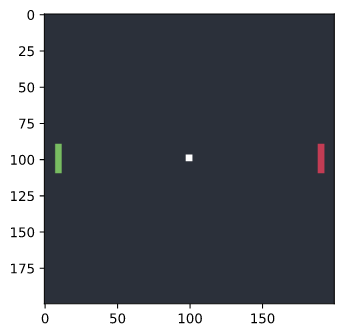
\includegraphics[width=\textwidth]{figures/raw.png}
        \caption{Raw 200x200 frame}
        \label{fig-raw}
    \end{subfigure}
    \begin{subfigure}{0.49\textwidth}
        \centering
        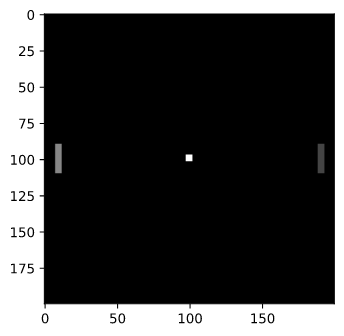
\includegraphics[width=\textwidth]{figures/bw.png}
        \caption{Black and White processed frame}
        \label{fig-bw}
    \end{subfigure}

    \begin{subfigure}{0.49\textwidth}
        \centering
        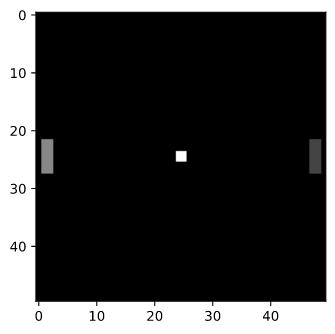
\includegraphics[width=\textwidth]{figures/small.png}
        \caption{Down Sampled 50x50 frame}
    \end{subfigure}
    \caption{Frame in different stages of processing}
    \label{fig-small}
    \label{fig-process}
\end{figure}

\subsection{DQN}
\label{sec:dqn-method}

Q-learning base algorithm shows the iterative update rule for an action value function, which is said to find optimality for any FMDP assuming infinite exploration.


$Q^{n e w}\left(s_{t}, a_{t}\right) \leftarrow(1-\alpha) \cdot \underbrace{Q\left(s_{t}, a_{t}\right)}_{\text {old value }}+\underbrace{\alpha}_{\text {learning rate }} \cdot \overbrace{(\underbrace{r_{t}}_{\text {reward }} +  \underbrace{\gamma}_{\text {discount factor }}\cdot \underbrace{\max_{a}Q\left(s_{t+1}, a\right))}_{\text{estimate of optimal future value}}}^{\text {learned value }}$

\noindent
With learning rate $\alpha$, reward $r_t$ for moving into $s_{t+1}$ from $s_t$ taking action $a$ and the discount factor $\gamma$, which controls how important the future rewards are, or how much into the future the model looks.\\

\noindent
On top of the basic algorithm, DQN is a functional approximation variant of the Q-learning, in which the model is supposed to be deep (more than one layer). We used a delayed network (updated every 20 episodes) to compute the delayed values and tried both GLIE epsilone-greedy as well as a linear decaying epsilone of the form of $\frac{5mil-SF}{5mil}$, with $SF$ being the total number of frames out of all episodes, and capped the it's minimum epsilon value to $\epsilon=0.1$. We noticed that having the model around episode 50k with about $50\%$ win-rate and $\epsilon=0.1$ actually worsened the model from that point onwards, so we capped $\epsilon$ to 0.3 untill episode 125000 and have it linearly decrease until 180000 (where it reached 0.1).\\


\noindent
Figure 2 shows the two main data augmentation/preprocessing we ended up doing for the dqn models. Aside from that, we also tried stacking them on a 3rd dimension, like the channels of an RGB image and have according convolution layers, but it seemed a little bit worse than putting the images on top of each other. \\

\noindent
Vertically stacked images with downscaling and gray-scaling, as described also in the "Preprocessing Pipeline", section 3. The idea behind leaving the right pallet blacked out, came after we noticed that the model was doing decently against simple-ai (around $60\%$ win-rate), while having around $50\%$ against Karpathy. Rendering it, we noticed that that the dqn model probably learned that it's highes action-values, are those that get it's pole into the same position as the simple-ai model (it was probably imitating it), and the 60\% (so "better" than simple-ai) was probably a mere consequence of the delay with which it went to catch the ball, catching it with the edge, speeding it up and winning a little be more often.\\

    \begin{minted}{python}
            Conv2d(channels, 32, kernel_size=(7, 7), stride=1)
            MaxPool2d(kernel_size=(2, 2))
            Conv2d(32, 32, kernel_size=(5, 5), stride=1)
            MaxPool2d(kernel_size=(2, 2))
			Linear(9792, 120)
			Linear(120, 3)
	\end{minted}

\noindent
The model architecture that ended up being good enough to beat simple-ai on 80\%+, was composed of two convolution layers, with max-pooling layers in between, followed by two linear layers, $9792x120$ and $120x3$:






\begin{figure}[!htb]
    \centering
    \begin{subfigure}{.49\textwidth}
        \centering
        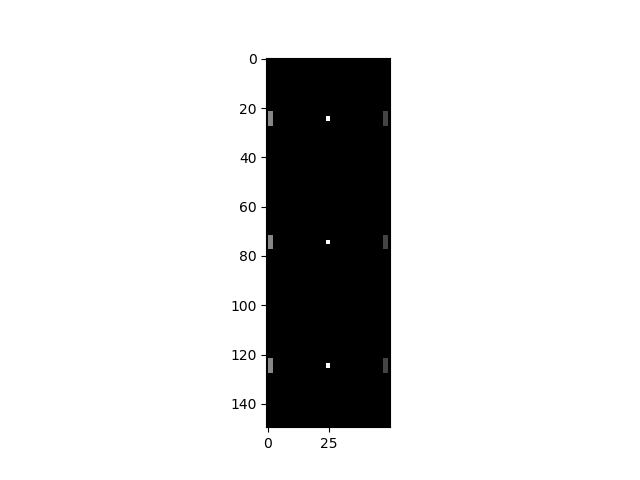
\includegraphics[width=\textwidth]{figures/dqn_training_image.png}
        \caption{Preprocessed 3-stacked images}
        \label{fig-raw}
    \end{subfigure}
    \begin{subfigure}{0.49\textwidth}
        \centering
        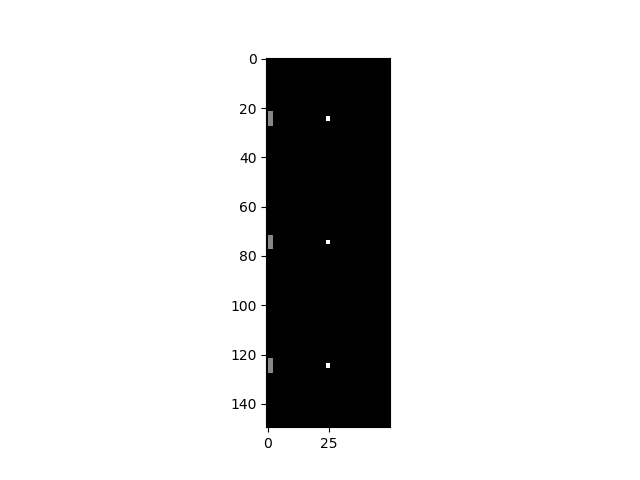
\includegraphics[width=\textwidth]{figures/dqn_training_image_blacked_out_pallet.png}
        \caption{Preprocessed 3-stacked images with blacked-out pallet}
        \label{fig-bw}
    \end{subfigure}
    \caption{DQN image augmentation and processing}
    \label{fig-small}
    \label{fig-process}
\end{figure}

\subsection{A3C}
\label{sec:a3c-method}
The policy gradient algorithm REINFORCE introduced in Sutton\&Barto \cite{Sutton1998} describes how the performance of the policy parameters $\theta$ denoted by $J(\theta)$ can be used to maximize the performance of the agent by moving the parameters in the direction of the gradient of $J(\theta)$.
\[
   \nabla J(\boldsymbol{\theta})= \mathbb{E}_{\pi}\left[ G_{t} \frac{\nabla \pi(A_{t}\mid S_{t},\boldsymbol{\theta})}{\pi(A_{t}\mid S_{t},\boldsymbol{\theta})} \right]  
\]
The parameter update then is given by 
\[ 
    \boldsymbol{\theta}_{t+1} = \boldsymbol{\theta}_{t} + \alpha G_{t}\frac{\nabla \pi(A_{t}\mid S_{t},\boldsymbol{\theta})}{\pi(A_{t}\mid S_{t},\boldsymbol{\theta})}
\]
The baseline addition to the REINFORCE algorithm is a neat mathematical trick to add to the policy gradient. As seen in \cite{Sutton1998},
\[
    \nabla J(\boldsymbol{\theta}) \propto \sum_{s} \mu(s) \sum_{a}\left(q_{\pi}(s, a)-b(s)\right) \nabla \pi(a | s, \boldsymbol{\theta})
\]
where $J(\theta)$ is the performance of the policy, $\mu(s)$ is the normalized time spent in each state. We see that the addition of a baseline term $b(s)$ doesn't not change the gradient as $    \sum_{a} b(s) \nabla \pi(a | s, \boldsymbol{\theta}) = 0$. This fact can then be used in the calculation of loss for the algorithm which doesn't change the expected value of the update. The benefit of the baseline then is to control the variance during training. 

\medskip
\noindent
The actor-critic model is just a baseline REINFORCE model where we also have an approximation of the value function that is then used as the baseline. Therefore we can use a TD(0) update to get an unbiased estimate of the value function in a particular episode. Hence the TD-error then can be called \textbf{advantage} considering a value function $\Hat{v}$ that shares the same parameters $\boldsymbol{\theta}$ as the policy approximation
\[ 
    \delta_{t,\boldsymbol{\theta}} = R_{t+1} +\gamma\Hat{v}(S_{t+1},\boldsymbol{\theta}) - \Hat{v}(S_{t},\boldsymbol{\theta})
\]
Then the policy gradient update step just looks like 
\[ 
    \nabla J(\boldsymbol{\theta}) \approx \mathbb{E}_{\pi}\left[ \nabla_{\boldsymbol{\theta}} \ln \pi_{\boldsymbol{\theta}}(A_{t}\mid S_{t},\boldsymbol{\theta})\delta_{t,\boldsymbol{\theta}} \right]   
\]
This gives us gradients with much less variance hence is a good signal for a neural network to learn a policy from. The paper on A3C \cite{A3C} explains how this process can be scaled to multiple parallel actor-learners , this process removes the need for experience replay to stabilize the learning, hence we can use the on-policy advantage actor-critic method. It also comes with the added benefit of speeding up the training byy running multiple processes. They explain how a common slow changing target network that get the shared gradients from the individual learners. 

\bigskip
\noindent
Although the theory for A3C is fairly straightforward implementing a working model from scratch is rarely trivial. Due to this fact we searched for existing \texttt{pytorch} implementations of A3C and found the repository of Kostrikov Ilya \cite{orig_a3c}, which had 3 convolution layers and a LSTM layer at the end that gives the model a temporal memory allowing it perform very good on Atari environments. This code base was still pretty complex and this lead to finding an easier repository of Sam Greydanus \cite{baby-a3c}, which had a light weight implementation using the multiprocessing module of \texttt{pytorch} to share model parameters across processes. using this as a base we were able to integrate the given Pong environment and preprocessing steps that was outlined in Section~\ref{subsec:processing}

The model has 4 convolution layers followed by a GRU (instead of LSTM as it performs the same and has fewer parameters) which is then used with individual linear layers to get a actor(policy) and critic value as seen in Listing~\ref{code-a3c-params}

\begin{listing}[ht]
    \begin{minted}{python}
        (conv1): Conv2d(1, 32, kernel_size=(3, 3), stride=(2, 2), padding=(1, 1)) 
        (conv2): Conv2d(32, 32, kernel_size=(3, 3), stride=(2, 2), padding=(1, 1))
        (conv3): Conv2d(32, 32, kernel_size=(3, 3), stride=(2, 2), padding=(1, 1))
        (conv4): Conv2d(32, 32, kernel_size=(3, 3), stride=(2, 2), padding=(1, 1))
        (gru): GRUCell(512, 256)
        (critic_linear): Linear(in_features=256, out_features=1, bias=True)       
        (actor_linear): Linear(in_features=256, out_features=3, bias=True)  
      \end{minted}
    \caption{A3C Model parameters}
    \label{code-a3c-params}
\end{listing}

The model is updated for every 20 timesteps and in those timesteps the GRU layer has it's hidden state propagated. This effectively translates into holding roughly 20 frames of information in the GRU's hidden layer. After 20 frames the hidden layer is detached from the computation graph and then the environment continues.
    

\subsection{Rewards}
The rewards are important in a RL framework as it sends the signals to the model that allow it to move towards an optimal policy. The particular set up we have we get very sparse rewards, when the agent wins after an episode it gets a reward of $+10$ and if it loses then it gets $-10$. As we have no access to the internal dynamics of the network we cannot engineer any features based on our knowledge of the domain of Pong. Further on we will refer to these rewards as \textbf{normal rewards}. 

\medskip
\noindent
Even though we mentioned that we have limited game dynamics to engineer rewards, we can still get the amount of time the agent stays alive. As most game agent goes, a basic heuristic is that the longer the agent stays alive the better chance it will have at winning. Utilizing this idea we came up with a couple of ideas to try. On a small note, we did end up finding out that not all rewards worked for all RL models.

\medskip
\noindent
The first idea we tried was to check how long the agent stays alive in total and factor that into the final reward structure. We dubbed this approach \textbf{time to death}(ttd), where we keep track of how long the episode lasts and doing a superficial analysis of distributution scaled it by 50 timesteps and added it with the normal rewards as seen below where $t$ is the time of the episode
\[
    R_{ttd} = \frac{t}{50} \pm 10 
\]
The issue we found with this reward is that it is still sparse and doesn't fix any issues that the normal rewards had. Having the reward being scaled by 50 also tends bias the agent to find fast strategies even when it wasn't possible.

\medskip
\noindent
In attempts to fix the ttd rewards we aimed at giving a small reward at every time step similar to the cartpole environment and also maintaining the final win/loss rewards. The idea behind it was that this small reward will help the agent to learn to stay alive long enough to get the large $\pm 10$ at the end of the episode. The value to be chosen also seemed to play a role as a large enough reward at every timestep could make the agent learn strategies to keep playing rather than winning against the opponent. Hence we decided to try values of $0.01$ and $0.05$ per timestep. We will call these reward structures as \textbf{0.05 Rewards} and \textbf{0.01 Rewards}. 

\medskip
\noindent
Honorable mentions of other ideas we tried were rewards such as $e^{-(t-50)^{2}}$ which did not prove successful as it restricts the rewards and tends to force suboptimal agent policies. We did have other rewards that didn't pan out, hence we will got into much details in the report.

\section{Results and Performance Analysis}
\label{sec:results}

\subsection{DQN}

\subsection{A3C}
Now we discuss the training and test results of the A3C model that was described in Section~\ref{sec:a3c-method}. The asynchronous method of running the training means that we are unable to train on the GPU. This however means we are able to use all the available CPU cores by running 20 processes which each collects training information. This along with the reduced size of the input frames means the speed-up we get is significant. We are able to process $100$K frames in as little as 1 minute.

\medskip
\noindent
From the training graphs we see in Figure~\ref{fig:a3c-training} that irrespective of the rewards we use the model trains really fast and is able to converge withing the $80$M frames we trained all the networks for, which takes only a single day. We can see that in Figure~\ref{fig:training-a3c-05} that the rewards seem to make the model train in the first couple of million frames very well. To further analyze the training performance refer to Figure~\ref{fig:a3c-training-close}.


\begin{figure}[ht!]
    \centering
    \begin{subfigure}{0.49\textwidth}
        \centering
        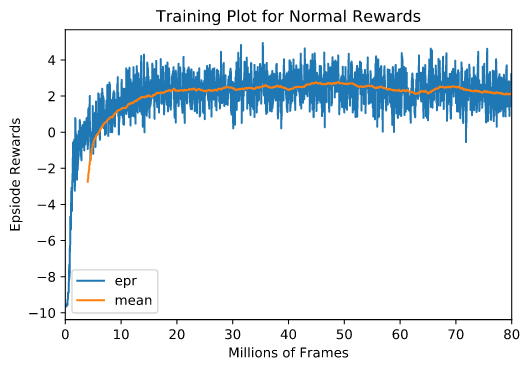
\includegraphics[width=\textwidth]{figures/a3c-training-normal.png}
        \caption{Normal Rewards}
        \label{fig:training-a3c-normal}
    \end{subfigure}
    \begin{subfigure}{0.49\textwidth}
        \centering
        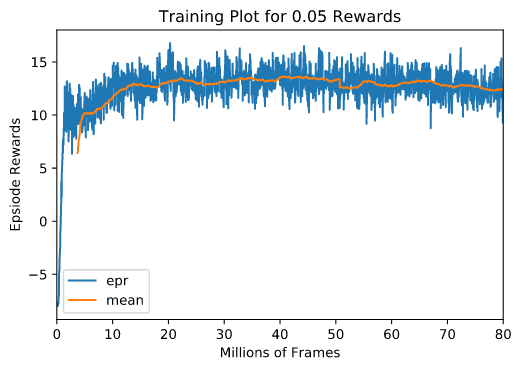
\includegraphics[width=\textwidth]{figures/a3c-training-0-05.png}
        \caption{Reward of $0.05$ for staying alive and $\pm 10$ at end}
        \label{fig:training-a3c-05}
    \end{subfigure}
    
    \begin{subfigure}{0.49\textwidth}
        \centering
        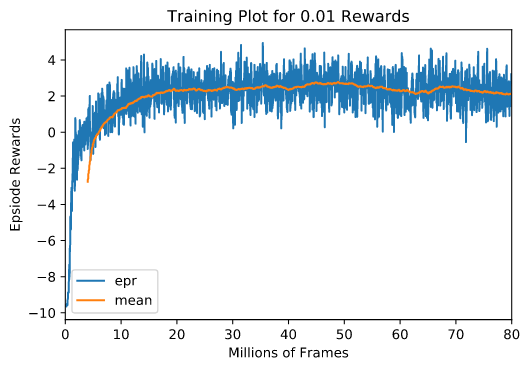
\includegraphics[width=\textwidth]{figures/a3c-training-0-01.png}
        \caption{Reward of $0.01$ for staying alive and $\pm 10$ at end}
        \label{fig:training-a3c-01}
    \end{subfigure}
    \caption{Training Graphs for a3C model with various rewards}
    \label{fig:a3c-training}
\end{figure}

Now looking at the first 10-12M frames in Figure~\ref{fig:a3c-training-close} we see the clear differences in the effect of the rewards used. There is one difference that has to be explained, is the range of the rewards that are from $-10$ to a varying range. This is because when providing a reward for staying alive, the model tends to stay alive in the 100s of timesteps, hence a reward of $0.01$ gives only $1$ accumulated compared to $5$ when it is $0.05$. Moving past this we see that the \textbf{normal rewards} takes longer to converge to a lower mean reward than the other two reward strategies, as see in Figure~\ref{fig:training-close-a3c-normal} and \ref{sub@fig:training-close-a3c-05}. We particularly see that for \textbf{0.05} rewards the learning rate is very fast reaching a mean reward of 10 by 2 million frames. 
\begin{figure}[ht!]
    \centering
    \begin{subfigure}{0.49\textwidth}
        \centering
        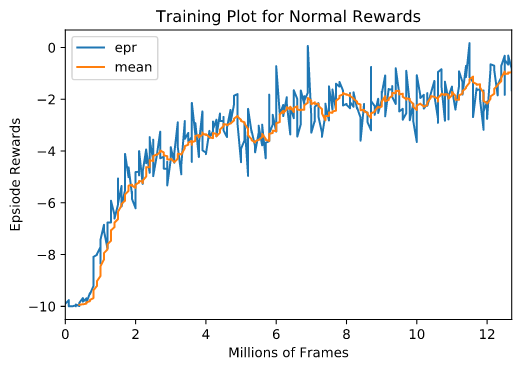
\includegraphics[width=\textwidth]{figures/a3c-training-normal_close.png}
        \caption{Normal Rewards}
        \label{fig:training-close-a3c-normal}
    \end{subfigure}
    \begin{subfigure}{0.49\textwidth}
        \centering
        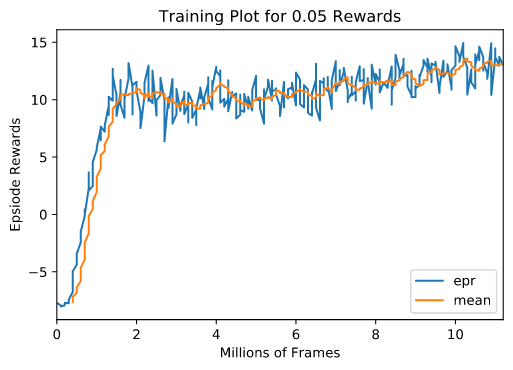
\includegraphics[width=\textwidth]{figures/a3c-training-0-05_close.png}
        \caption{Reward of $0.05$ for staying alive and $\pm 10$ at end}
        \label{fig:training-close-a3c-05}
    \end{subfigure}
    
    \begin{subfigure}{0.49\textwidth}
        \centering
        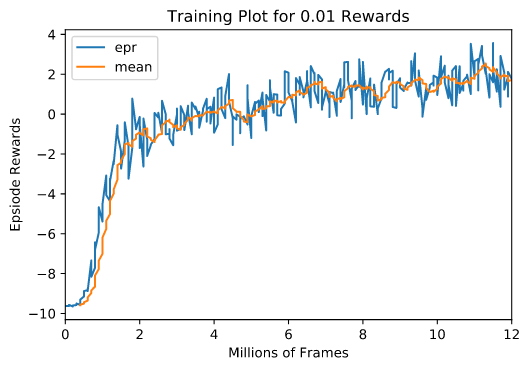
\includegraphics[width=\textwidth]{figures/a3c-training-0-01_close.png}
        \caption{Reward of $0.01$ for staying alive and $\pm 10$ at end}
        \label{fig:training-close-a3c-01}
    \end{subfigure}
    \caption{Closer look of training Graphs for a3C model with various rewards}
    \label{fig:a3c-training-close}
\end{figure}

Although training rewards are a good indicator of whether a model is training correctly or not, it is not necessarily an indicator of how well it will perform when tested against the SimpleAI which it trained against or other agents provided in the \texttt{test\_bench} code. We take the model saved at various stages of training till around 50 million frames and test it against 4 agents for 200 games. Due to the games being slightly random, this still provides a good estimate of the performance of the model. The results are seen in Figure~\ref{fig:a3c-testing}.

\medskip
\noindent
The most interesting results are those in Figure~\ref{fig:test-a3c-simpleai} which is the agent that we originally trained against. We see that there is some overfitting is happening as we move closer to 50 Million frames. To get a better idea we have Figure~\ref{fig-a3c-testing-simpleai-closer} where we look at the models till 20 million frames. We see that all the models start out at nearly 50\% win rate at 2 million frames. Then we see that the models that have rewards for staying alive, i.e. $0.01$ and $0.05$ rewards have better win rates. By 10 million frames the $0.01$ model achieves nearly 90\% win rate. We see in this time that the \textbf{normal rewards} are slower to converge to a better win rate, always behind the other 2 models. As we come to the 20 million mark zone we see this trend reversing, the $0.01$ and $0.05$ models start to overfit and the performance degrades to a win rate of high 80\% even see in Figure~\ref{sub@fig:test-a3c-simpleai}. After 20M frames the normal rewards model catches up and performs as well. This means that we need to stop training earlier for the other models.

\medskip
\noindent
From the perform against other agents we also see a similar trend, the normal rewards model takes longer to achieve the same performance but eventually by 50M frames outperforms the other models. This is clearly seen against \textit{SomeAgent} in Figure~\ref{sub@fig:test-a3c-someagent}. This confirms that the $0.01$ and $0.05$ rewards tend to overfit very soon. A thing to notice is that the model performs near optimally with 90\% win-rate against other models. This clearly indicates that the model has learnt to generalize well. 
\begin{figure}[th!]
    \centering
    \begin{subfigure}{0.49\textwidth}
        \centering
        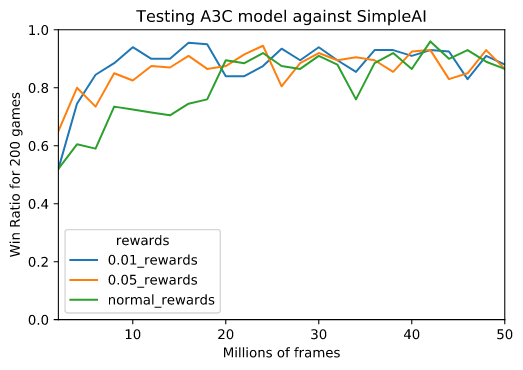
\includegraphics[width=\textwidth]{figures/a3c-test-simpleai.png}
        \caption{Against SimpleAI}
        \label{fig:test-a3c-simpleai}
    \end{subfigure}
    \begin{subfigure}{0.49\textwidth}
        \centering
        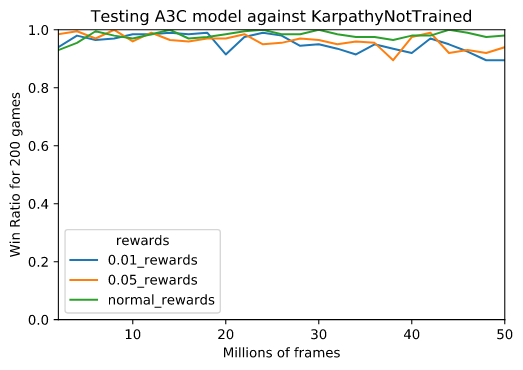
\includegraphics[width=\textwidth]{figures/a3c-test-karpathy-not-trained.png}
        \caption{Against KarpathyNotTrained}
        \label{fig:test-a3c-karpathy}
    \end{subfigure}

    \begin{subfigure}{0.49\textwidth}
        \centering
        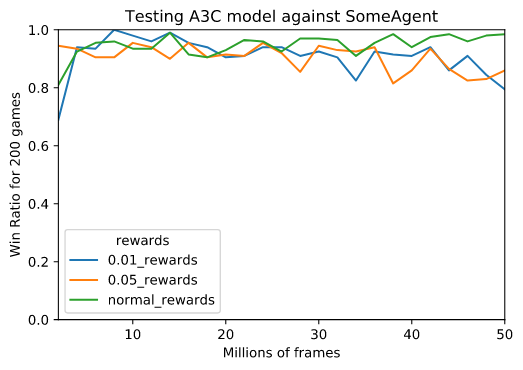
\includegraphics[width=\textwidth]{figures/a3c-test-someagent.png}
        \caption{Against SomeAgent}
        \label{fig:test-a3c-someagent}
    \end{subfigure}
    \begin{subfigure}{0.49\textwidth}
        \centering
        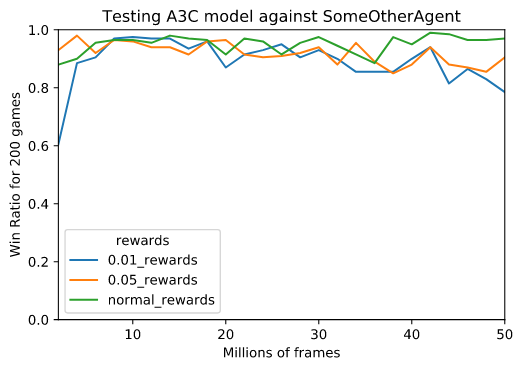
\includegraphics[width=\textwidth]{figures/a3c-test-someaothergent.png}
        \caption{Against SomeOtherAgent}
        \label{fig:test-a3c-someotheragent}
    \end{subfigure}
    
    \caption{Test of A3C model against agents}
    \label{fig:a3c-testing}
\end{figure}

\begin{figure}[ht!]
    \centering
    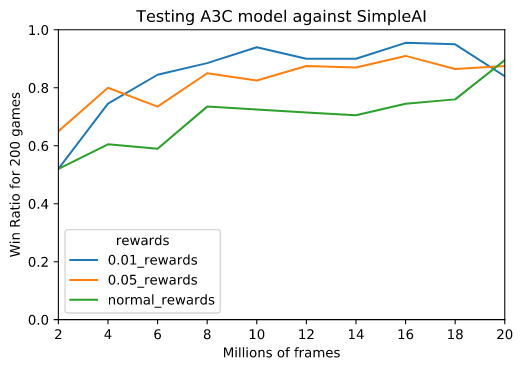
\includegraphics[width=0.5\textwidth]{figures/a3c-test-simpleai-close.png}
    \caption{Closer look at SimpleAI test results}
    \label{fig-a3c-testing-simpleai-closer}
\end{figure}

\section{Conclusions}
\label{sec:conclusion}

\section{Acknowledgements}
We would like to thank Dimitrios Papatheodorou, Abhilash Jain, Maxim Afteny and others with whom we discussed and brainstormed ideas and methods to implement in this project.
\clearpage      
\bibliography{ref}{}
\bibliographystyle{plain}
\end{document}